\documentclass[a4]{article}

\usepackage{tikz}
\usepackage{luatexja}
\usepackage[table]{xcolor} %表のセルに色をつけるため
\usepackage{diagbox} %表の斜め線を引くため


%表のセル書式:中央寄せ+幅指定
\newcolumntype{C}[1]{>{\centering\arraybackslash}p{#1}}

\begin{document}

%折れ線グラフ
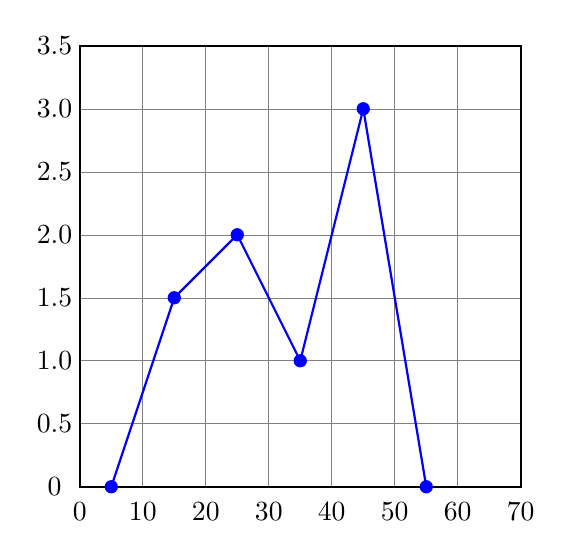
\begin{tikzpicture}[scale=0.8]
  %グリッド
  \draw[step=1cm,gray,very thin] (0,0) grid (7,7);

  %枠
  \draw[thick] (0,0)--(7,0)--(7,7)--(0,7)--cycle;

  % 棒グラフ(長方形)
  %\fill[blue!70] (0.5,0) rectangle (1.5,3);
  %\fill[red!70]  (2.0,0) rectangle (3.0,4.5);
  %\fill[green!70](3.5,0) rectangle (4.5,2.5);
  %\fill[orange!80](5.0,0) rectangle (6.0,1.5);

  %横軸ラベル
  \node at (0,-0.4) {0};
  \node at (1.0,-0.4) {10};
  \node at (2.0,-0.4) {20};
  \node at (3.0,-0.4) {30};
  \node at (4.0,-0.4) {40};
  \node at (5.0,-0.4) {50};
  \node at (6.0,-0.4) {60};
  \node at (7.0,-0.4) {70};
  
  %縦軸ラベル
  \node at (-0.4,0) {0};
  \node at (-0.4,1) {0.5};
  \node at (-0.4,2) {1.0};
  \node at (-0.4,3) {1.5};
  \node at (-0.4,4) {2.0};
  \node at (-0.4,5) {2.5};
  \node at (-0.4,6) {3.0};
  \node at (-0.4,7) {3.5};
  
  %点
  \coordinate (A) at (0.5,0);
  \coordinate (B) at (1.5,3);
  \coordinate (C) at (2.5,4);
  \coordinate (D) at (3.5,2);
  \coordinate (E) at (4.5,6);
  \coordinate (F) at (5.5,0);
  
  \fill[blue] (A) circle (3pt);
  \fill[blue] (B) circle (3pt);
  \fill[blue] (C) circle (3pt);
  \fill[blue] (D) circle (3pt);
  \fill[blue] (E) circle (3pt);
  \fill[blue] (F) circle (3pt);
  
  \draw[blue,thick] (A)--(B)--(C)--(D)--(E)--(F);
\end{tikzpicture}


\bigskip


%度数分布のグラフ
\begin{tikzpicture}
  %横線グリッドだけ(Y方向に水平線)
  \foreach \y in {1,2,3,4,5} {
    \draw[cyan, very thin] (0,\y) -- (6,\y);
  }
  
  %枠線
  \draw[cyan,thick] (0,0) -- (6,0)--(6,6)--(0,6)--cycle;
  
  %棒グラフの棒
  \draw[blue,thick,fill=blue!30] (0.5,0) rectangle (1.5,2);
  \draw[blue,thick,fill=blue!30] (1.5,0) rectangle (2.5,3);
  \draw[blue,thick,fill=blue!30] (2.5,0) rectangle (3.5,5);
  \draw[blue,thick,fill=blue!30] (3.5,0) rectangle (4.5,1);
  
  %折れ線グラフ
  \coordinate (A) at (1,2);
  \coordinate (B) at (2,3);
  \coordinate (C) at (3,5);
  \coordinate (D) at (4,1);
  \coordinate (E) at (5,0);
  \fill[red] (A) circle (2pt);
  \fill[red] (B) circle (2pt);
  \fill[red] (C) circle (2pt);
  \fill[red] (D) circle (2pt);
  \fill[red] (E) circle (2pt);
  \draw[red,thick] (A)--(B)--(C)--(D)--(E);

  %横軸ラベル
  \node at (0.5,-0.3) {$10$};
  \node at (1.5,-0.3) {$15$};
  \node at (2.5,-0.3) {$20$};
  \node at (3.5,-0.3) {$25$};
  \node at (4.5,-0.3) {$30$};
  \node at (5.5,-0.3) {$35$};
  \node at (6.5,-0.3) {(m)};
  
  %縦軸ラベル
  \node at (-0.3,0) {$0$};
  \node at (-0.3,1) {$2$};
  \node at (-0.3,2) {$4$};
  \node at (-0.3,3) {$6$};
  \node at (-0.3,4) {$8$};
  \node at (-0.3,5) {$10$};
  \node at (-0.3,6) {$12$};
  \node at (-0.3,6.6) {(人)};
  
  %タイトル
  \node at (3,6.6) {\large ハンドボール投げの記録};
\end{tikzpicture}

\bigskip

%相対度数表
\renewcommand{\arraystretch}{2} %セルの高さを1.5倍に
\setlength{\arrayrulewidth}{1pt} %表全体の線の太さ
\begin{tabular}{|C{2cm}|C{1.5cm}|C{2cm}|C{2cm}|} %プリアンブルで指定した書式
  \hline
  \large 階級 & \large 度数 & \large 累積度数 & \large 相対度数 \\
  \hline
  \ 0 \ ~ \ 10 & 2 & 2 & 0.2 \\
  \hline
  10 \ ~ \ 15 & 1 & 3 & 0.1\\
  \hline
  15 \ ~ \ 20 & 5 & 8 & 0.5\\
  \hline
  20 \ ~ \ 25 & 2 & 10 & 0.2\\
  \hline
  合計 & 10 & \cellcolor{gray}\rule[0.3em]{5mm}{1pt} & 1 \\ %\rule[文字の高さ]{長さ}{太さ}
  \hline
\end{tabular}

\bigskip

%曲線でラベルの両端を結ぶ
\begin{tikzpicture}
  % 点
  \coordinate (A) at (0,0);
  \fill (A) circle (2pt) node[left] {A};

  % ラベル
  \node[anchor=west] (label) at (3,1.5) {曲線でつながれたラベル};

  % ラベルの左右端
  %   label.west → 左端
  %   label.east → 右端
  
  %ベジェ曲線で結ぶ方法
  %\draw (始点) .. controls (始点側の制御点) and (終点側の制御点) .. (終点);

  % 曲線A→左端
  \draw[blue, thick] (A) .. controls +(1,1) and +(-1,0) .. (label.west);

  % 曲線A→右端(少し違う曲線)
  \draw[red, thick] (A) .. controls +(-1,-2) and +(1,1) .. (label.east);

  % 制御点がわかるようにラベルの枠をつける
  \draw[dashed, gray] (label.north west) rectangle (label.south east);
\end{tikzpicture}

\bigskip


%線分の長さの表し方
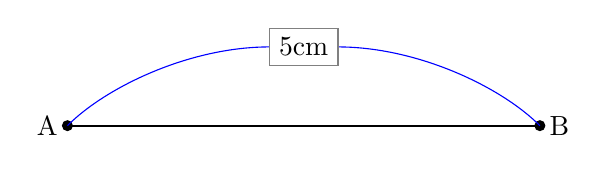
\begin{tikzpicture}
\coordinate (A) at (0,0);
\coordinate (B) at (6,0);
\fill (A) circle (2pt) node[left] {A};
\fill (B) circle (2pt) node[right] {B};
\draw[thick] (A)--(B);
%ラベル
\node (label) at (3,1) {5cm};
  
%ベジェ曲線で結ぶ
\draw[blue] (A) .. controls +(0.5,0.5) and +(-1,0) .. (label.west);
\draw[blue] (B) .. controls +(-0.5,0.5) and +(1,0) .. (label.east);

%ラベルの枠
\draw[gray] (label.north west) rectangle (label.south east);
\end{tikzpicture}

\end{document}
